\section{Corrientes relacionadas}

Los juegos serios son el solapamiento de tres corrientes, los juegos, las
técnicas de enseñanza y la simulación educativa\cite{education:games}, tal y
como se observa en la figura~\ref{fig:corrientes_relacionadas}. 

\begin{figure}[ht]
\centering
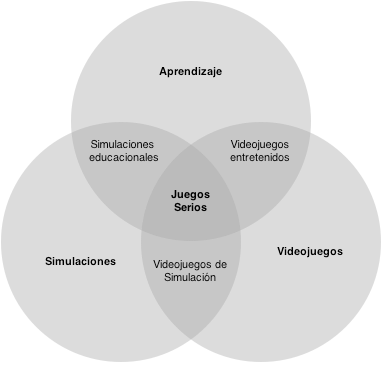
\includegraphics[scale=0.5]{juegos_serios/corrientes_paralelas.png}
\caption{Ubicación de los juegos serios entre los juegos, la simulación y la educación}
\label{fig:corrientes_relacionadas}
\end{figure}

Cuando se utilizan aspectos de juegos con simulaciones, se obtienen juegos, cuyo
objetivo es entretener mientras son similares a la realidad, dentro de esta
categoría podemos encontrar juegos como \emph{Gran Turismo}\revisar{Que
    divague}, si mezclamos factores relacionados al aprendizaje y a las
simulaciones se obtienen simulaciones sin interacción con el usuario que buscan
mostrar o enseñar como se comportan distintos fenómenos físicos, sociales, etc.


\subsection{Simulaciones educativas}

La simulación se define como el proceso de diseñar un modelo de un sistema real
y, llevar a cabo experimentos con este modelo, con el fin o bien de entender el
comportamiento del sistema o de la evaluación de distintas estrategias para la
operación del sistema\cite{ingalls2008introduction}. 

Un juego y una simulación podrían llegar a ser muy parecidos, a veces los juegos
tienen motores de simulación\footnote{Un motor de simulación es un conjunto de
    objetos y métodos que se utilizan para la construcción de modelos de
    simulación que están dentro de las aplicaciones}, una de las diferencias es
que la simulación es muy dependiente del contexto. 

La simulación en el ámbito de la educación fue evolucionando desde simples
motores de reglas hasta complejos entornos, la simulación demostró ser una
herramienta muy útil en el ámbito laboral\cite{mariluz:seiousgames}, pues enseña
al \fixme{alumno}{O usuario?, por que habla del ámbito profesional} a encarar
situaciones muy difíciles de representar en entornos completamente controlados y
provee mecanismos para comprobar la efectividad de la herramienta. 

Actualmente la simulación se utiliza más en el ámbito empresarial pues las
empresas son las más necesitadas de innovar en el ámbito de la enseñanza. Un
ejemplo de esta necesidad se da, por ejemplo, en el entrenamiento de nuevos
vendedores, es muy difícil enseñar a un vendedor como debe vender los productos
con un pizarrón y/o una presentación, en cambio la simulación permite que el
mismo pueda probar cosas nuevas y experiencias de sus compañeros (o instructor),
convirtiendo así el aprendizaje en colectivo\cite{mariluz:seiousgames}. En el
ámbito académico la simulación es más utilizada en campos físicos (como
simulación de fluidos), meteorología (simulación de tormentas y fenómenos
climáticos), etc. 

Existen dos tipos de simulaciones, en primer lugar están las experimentales que
ponen al estudiante en el lugar de un profesional y requieren que el mismo tome
decisiones para alcanzar los objetivos y en segundo lugar están las simbólicas
que buscan que el estudiante deduzca eventos, principios y mejores
prácticas\cite{charsky:2010}. 


\subsubsection{Partes de una simulación}

Una simulación esta conformada por:
\observacion{Ver si realmente hace falta explicar esto acá, o dejar para el
    capítulo de solución}

\begin{itemize}

\item \textbf{Entidades} Cualquier objeto o componente en el sistema que
    requiera representación explícita en el modelo se define como
    entidad\cite{banks2000dm}. Las entidades poseen atributos. Los atributos son
    las características de una determinada entidad que son exclusivos de esa
    entidad. Por último, son aquellas que cambian el estado de una simulación.
    Ejemplo de entidades son: un médico o una jeringa en una simulación médica.

\item \textbf{Acciones} Las entidades interactúan entre sí a través de acciones.
    Estas acciones puede causar cambios en el estado de la simulación además de
    eventos. Ejemplo de una acción en una simulación médica es la esterilización
    de un instrumento.

\item \textbf{Eventos} Los eventos son hechos que ocurren de manera controlada
    pero no siempre predecible en el entorno simulado, los mismos afectan a las
    entidades y deben obligar a realizar alguna de las acciones disponibles para
    tal evento. Ejemplo de un evento en un simulación médica es un paro cardíaco
    del paciente.

\end{itemize}


\subsubsection{Confianza en una simulación}

La confianza en el modelo o la simulación según\cite{DoDSysEng2001} se establece
mediante:

\begin{itemize}

\item \textbf{La verificación:} Es el proceso de determinar si la implementación
    representa con precisión las especificaciones del diseño. 

\item \textbf{La validación:} Es el proceso de determinar el grado en el que el
    modelo representa de forma exacta la realidad de acuerdo al uso que se tiene
    previsto darle y el nivel de confianza que debe tenerse en la evaluación.

\item \textbf{La acreditación:} Es el proceso de certificación de un modelo para
    su uso con un propósito específico.

\end{itemize}


\subsection{Diferencia entre juegos serios, simulaciones y mundos virtuales}

Estas tres alternativas son entornos virtuales altamente interactivas, todos con
sus propias posibilidades y fines. Los tres pueden ser similares
pero con las siguientes diferencias\cite{education:games}:

\begin{itemize}
\item \textbf{Simulaciones educativas}: utilizan escenarios rigurosamente
    estructurados con un conjunto altamente refinado de normas, retos y
    estrategias que son cuidadosamente diseñados para desarrollar las
    competencias específicas que se pueden transferir directamente al mundo
    real.
\item \textbf{Videojuegos:} son actividades atractivas y divertidas que
    habitualmente se utilizan exclusivamente para el entrenamiento pero también
    permiten una exposición con un conjunto determinado de herramientas,
    argumentos o ideas. Todas las partidas se juegan en un mundo estructurado
    por normas específicas, mecanismos de retroalimentación, y las herramientas
    necesarias, aunque no están tan definidas como en las simulaciones.
\item \textbf{Mundos virtuales:} son entornos sociales 3D multijugador, pero sin
    el enfoque en un objetivo en particular, como avanzar al siguiente nivel o
    navegar con éxito el escenario.
\end{itemize}
